% This is the section of the results focused on the assembly


\chapter{Transcriptome Assembly}

\section{Assembly Quality}

\subsection{Quality Statistics}


A primary motivation for the assembly and subsequent annotation has been the amount of data(reads) that are accounted for in the existing/reference annotation. An average of 1.7 million reads per sample are accounted for in these regions, out of an average of 10[M]illion rRNA-free reads.  Only 17\% of the usable, quality data are accounted for by the coding sequences of the reference annotation. However, 10M reads exceeds the typical sample depth for comparable efforts of transcript boundary identification. For these reasons, transcriptome assembly is necessary for transcript boundary identification.

4177 transcripts (7.18Mb from a 8.3Mb genome) were assembled, after removing duplicates. Each of these transcripts aligned to one location in the genome with \textgreater 98\% identity and less than 30bp of gaps. Of these, 1057 transcripts spanning 4.56Mb (25\% by the number of assembled transcripts;  63.5\% by assembled basepairs) contain 3287(86\%) reference ORF or one of 60 novel CDSes.  The remaining 3120 (75\% by number, 36.5\% by basepairs) of transcripts are novel (Fig. 1. Orange) and their lengths range from 200-32.7kb. The reference-ORF containing transcripts will be referred throughout as the ``standard'' set of transcripts and most of the investigation below describes this group.

The standard set of transcripts were larger on average by approximately an order of magnitude.

\begin{figure}
\begin{center}
\begin{minipage}[b]{2.25in}
\resizebox{2.25in}{2.5in}{
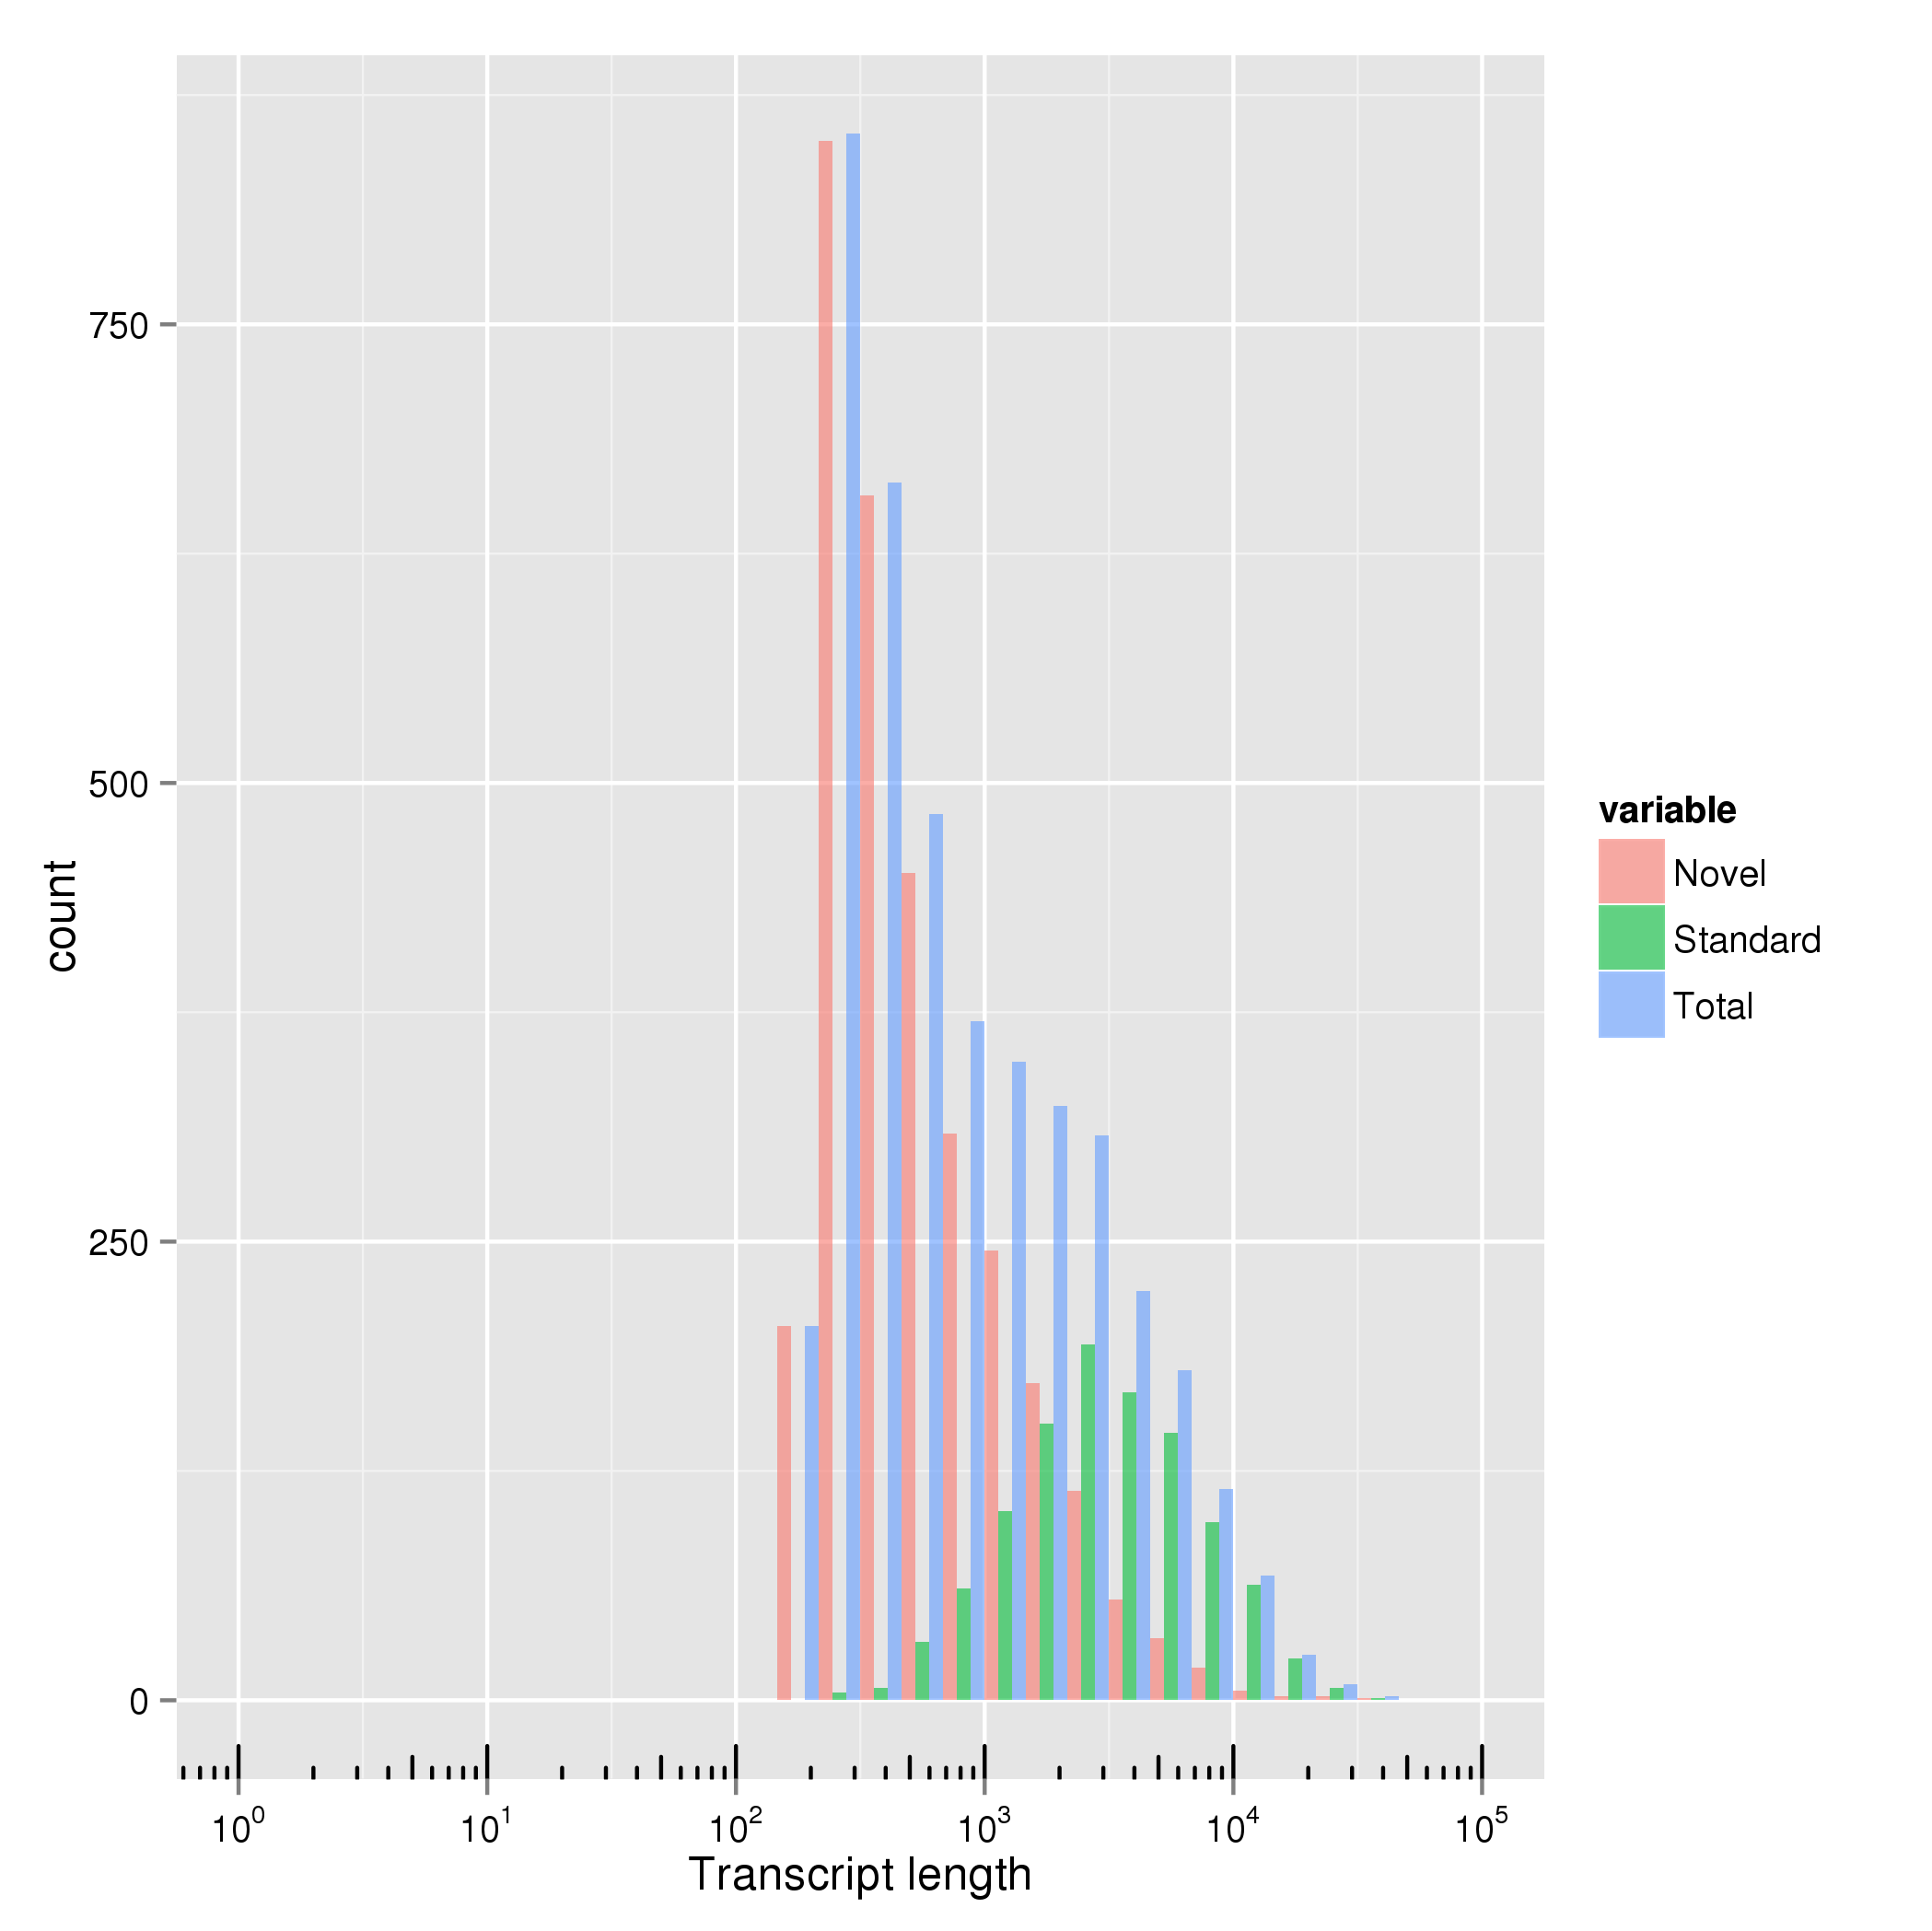
\includegraphics{images/Assembly/Summary/ftranscript_length.png}

}

\end{minipage}

\begin{minipage}[b]{2.25in}
\resizebox{2.25in}{2.5in}{
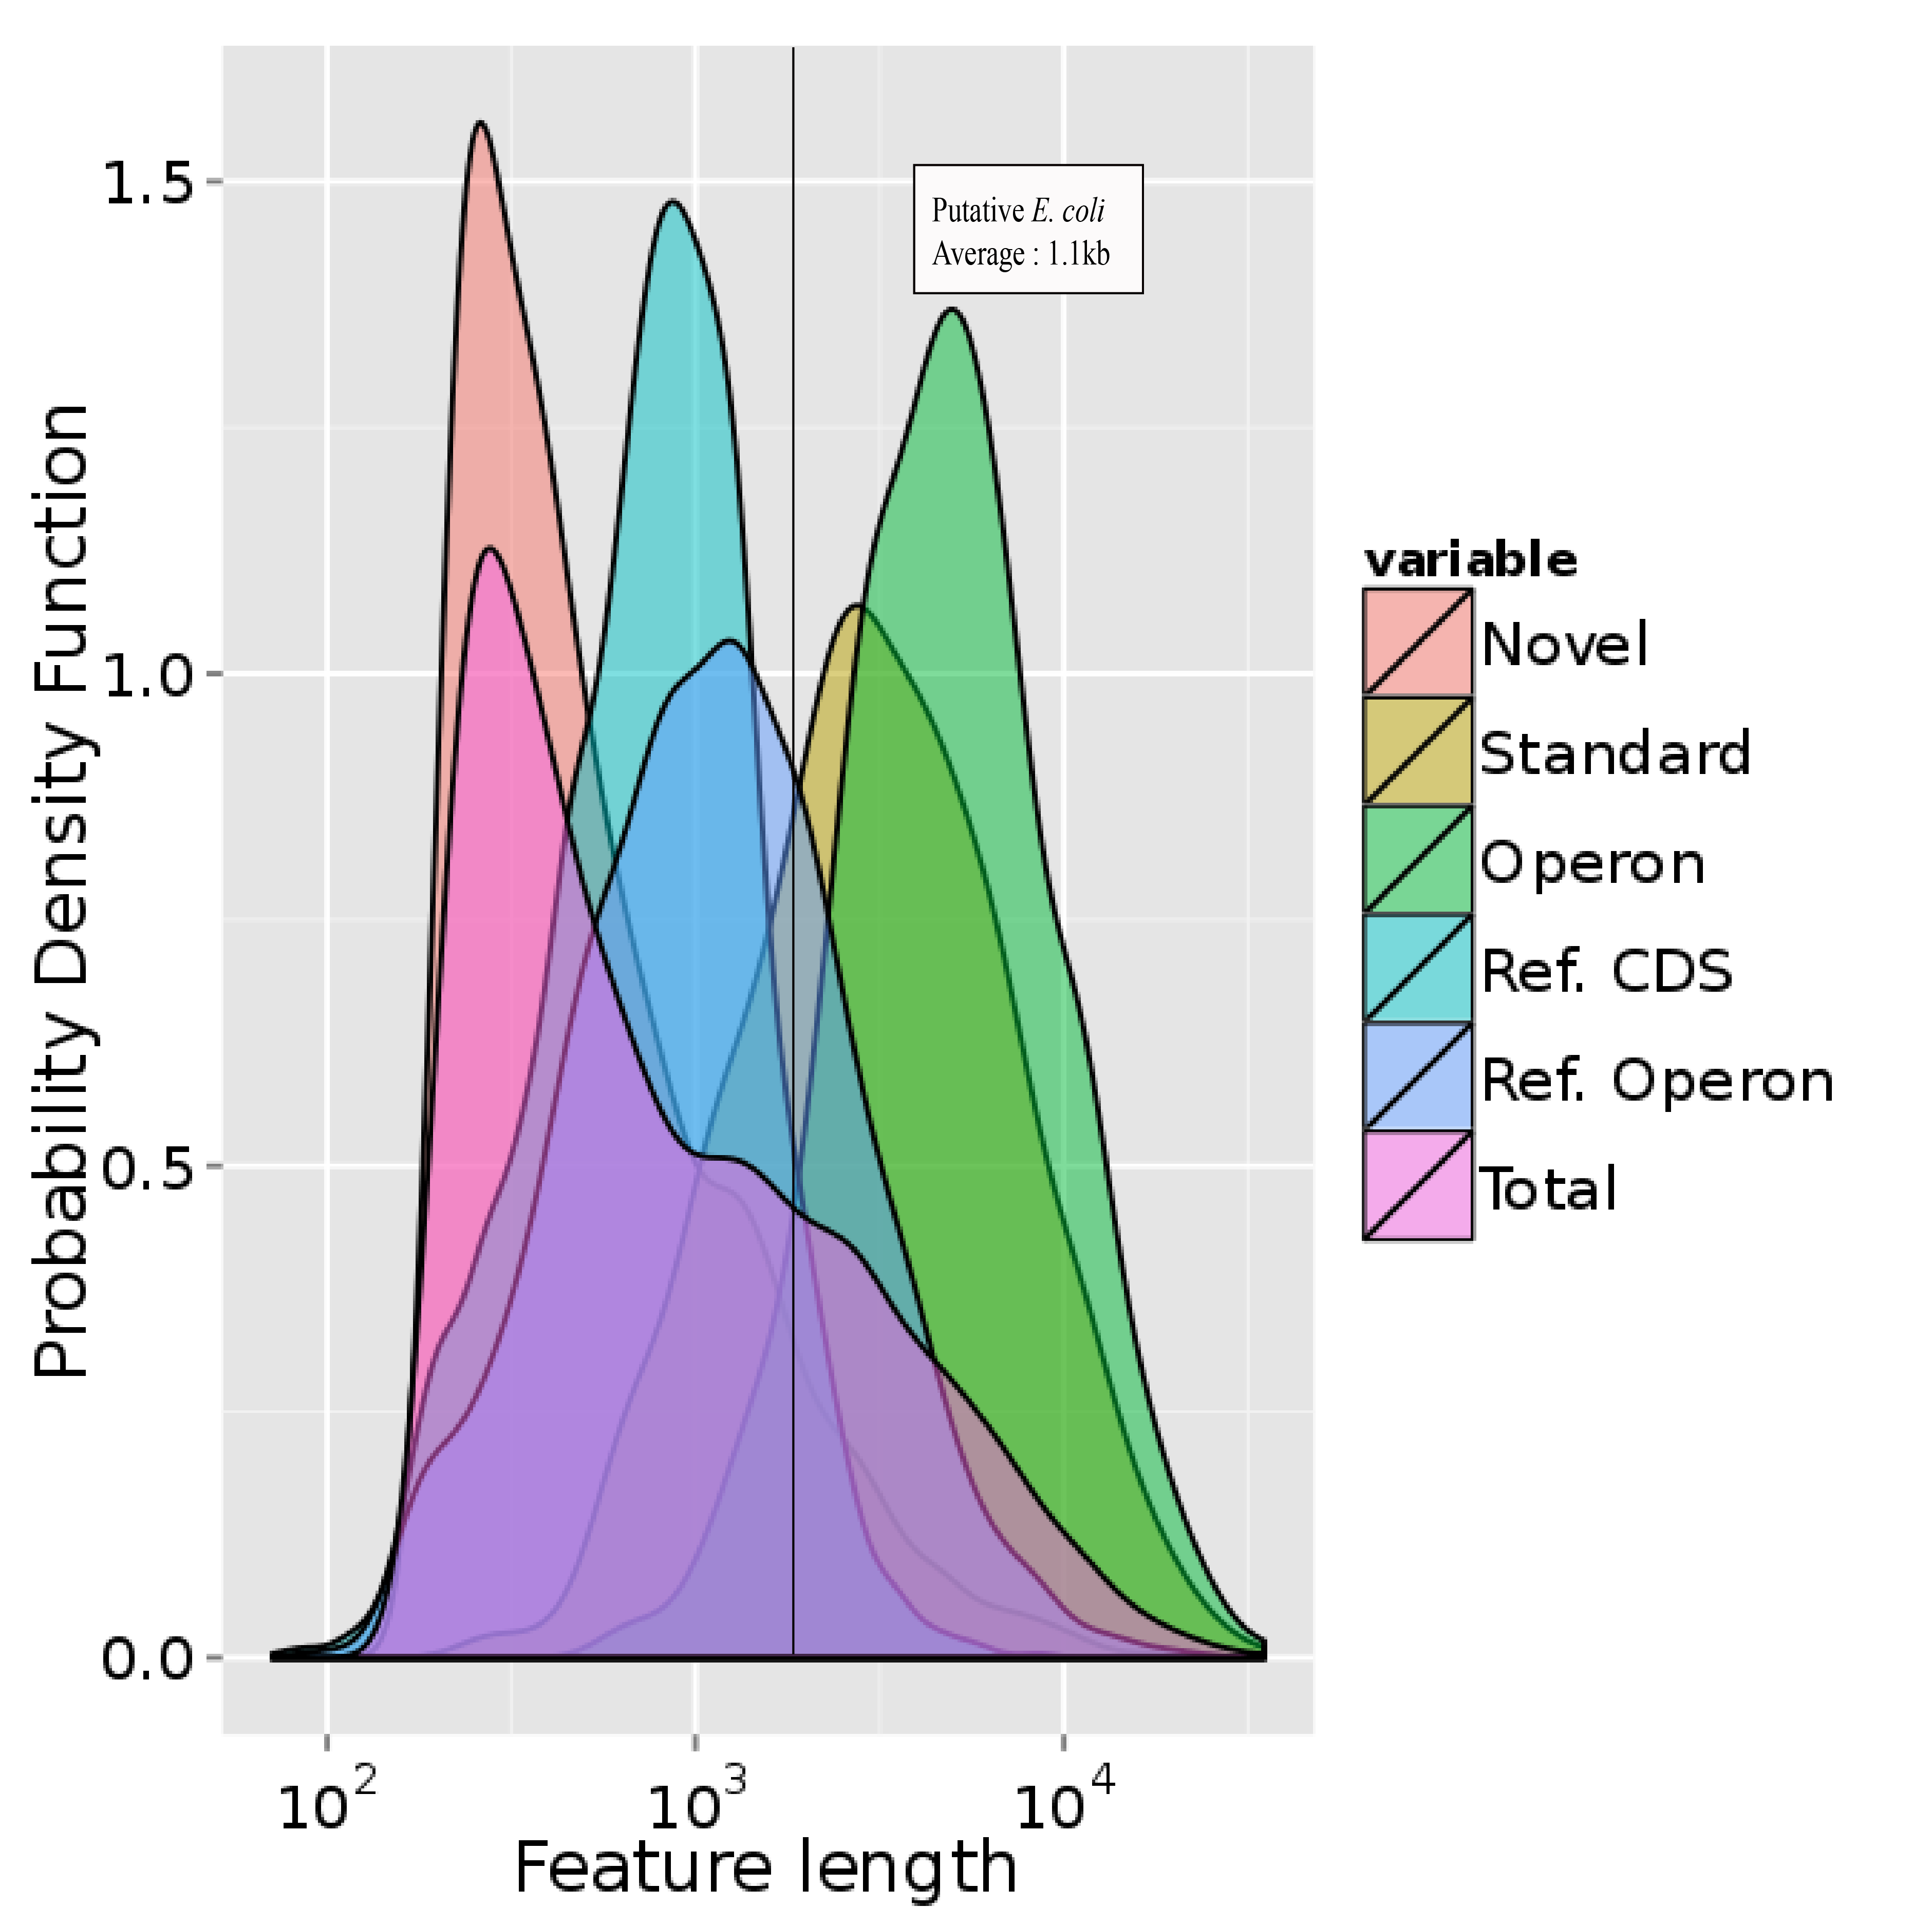
\includegraphics{images/Assembly/Summary/ffeature_length_1.png}
}

\end{minipage}
\end{center}

\caption{Transcript and Feature Length Distributions}
\end{figure}




\subsection{Example Transcripts}


To assess the data/assembly quality further, I used canonical transcripts of \textit{C. acetobutylicum}, to understand the agreement of the coverage, the assembly, and the existing annotation. Six issues, listed below, were considered for each example to better understand the quality of the assembly and the degree of curation required. 

\begin{enumerate}
\item Is the transcript large enough to include the known ORFs and RBSes?
\item Does the assembled transcript's TSS agree with promoter motifs?
\item Does it agree with published transcription start sites?
\item Does the assembled transcript's size agree with published Northern blots?
\item Does the assembly represent the coverage and if not, which of these two best represents the biological knowledge of this region?
\item Does the assembled region require curation (e.g. fused, extended, or truncated transcripts)?
\end{enumerate}

Agreement between the data and the literature would support the efficacy of this technique. Its effectiveness is particulary important in cases where no previous experimental data exists. These results could be very useful to future studies if only minimal remediation or curation is required. The first example that I examine is the Sol locus.

\subsubsection{Sol Locus}

The Sol locus is a 7kb region on the pSol1 megaplasmid surrounding the Sol operon(4.3kb, basepairs 175,564-179,841). This region is responsible for the production of several solvents\cite{62,63}. This region encodes several enzymes including a tri-functional NAD(H\textsuperscript{+})-dependent alcohol/aldehyde dehydrogenase (AdhE)\cite{62}, two subunits of coenzyme-A transferases (ctfA/B)\cite{66}, and an acetoacetate decarboxylase (Adc)\cite{64,65,66}. The region is also home to a protein SolR, which includes a helix-turn-helix motif and is thought to regulate solventogenesis\cite{67}. These genes are vital for carboxylic acid reuptake and conversion into alcohols, a vital part of this organism's metabolism and the solventogenesis process.

%          SOL LOCUS Fig 1.
\begin{figure}
\small
{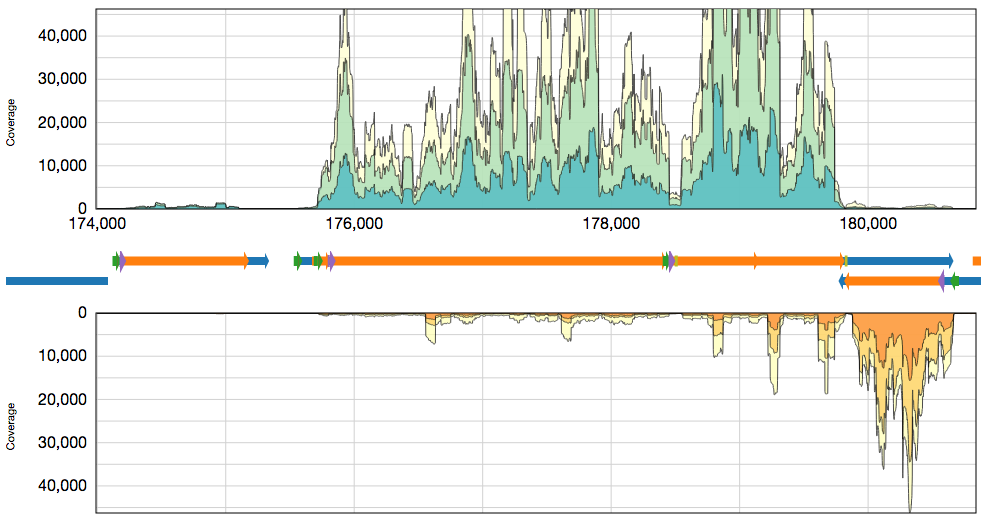
\includegraphics[width=\textwidth,height=2.5in]{images/Assembly/Examples/Sol/Sol-locus.png}
\subcaption{Sol locus}\label{fig:1a}}
% \label{fig:1}
\caption{Sol Locus Overview} This operon (\subref{fig:1a}) upper track) consists of OrfL, alcohol dehydrogenase (AdhE), and Co-A transferases A and B (ctfA,ctfB). SolR (far left) and acetoacetate decarboxylase (ADC; \subref{fig:1a} lower track, right) are also shown. Coverage for the Watson and Crick strands (top and bottom tracks) are visualized with an annotation track (center). Tracks show cumulative coverage for unstressed (yellow), butanol (light green/ light orange), and butyrate (green/orange) stressed samples over all time points. Transcripts (blue), ORFs (orange), RBSes (purple), inverted repeats (yellow), promoters (green), and TSSes (red) are represented as arrows and bars.
\end{figure}

\paragraph{Acetoacetate Decarboxylase Transcript}
In the early 1990s, several articles were published about the Sol locus including the cloning and sequencing of Adc and the Sol locus\cite{62,63,64,65,66}. An early study of the Sol operon probed the Adc locus, reporting two transcript sizes of 670 and 865 with Northern blot\cite{65}. The authors also reported the major transcription start site of Adc at base 180671 of the pSol1 plasmid. To examine the quality of our data and raw assembly, we examined this locus to observe the transcript size and locate the transcription start site in our data. In \ref{fig:2a} we see the transcription start site reported by Durre(red) located very near a sustained increase in sequencing coverage just downstream of a canonical promoter motif. This pattern of coverage (cumulatively \textgreater 10,000x) is sustained until a bidirectional Rho-independent terminator (\ref{fig:2b}). In this instance, the precise transcription start site was not estimated precisely by the uncurated assembly. The reported transcript continues for several hundred basepairs upstream of the Adc TSS, despite the decrease in coverage. This artifact is most likely due to sufficient k-mer complexity in the reads mapping upstream of the TSS for the Adc transcript to be fused to signal from genes upstream. Correcting for this error (\ref{fig:2c}), the full transcript size is 857. It was claimed that the 670bp product is most likely a specific degradation product or the result of a secondary transcriptional start site\cite{65}. To investigate this, a transcript of this size would correspond to a transcriptional start site at approximately base 180,484. Unfortunately, none of the promoter motifs in the region could explain a transcript of this size in vegetative cells. After curation based on the coverage pattern, promoter and terminator motifs in this region, the transcription start site and transcript size for Adc accurately match previous results. 

\begin{figure}
\small
{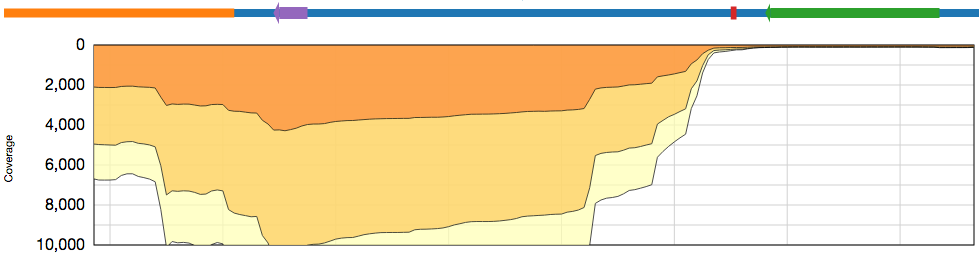
\includegraphics[width=\textwidth,height=1.5in]{images/Assembly/Examples/Sol/Sol-Adc-TSS.png}
\subcaption{Adc transcription initiation region on the Crick strand.}\label{fig:2a}}
{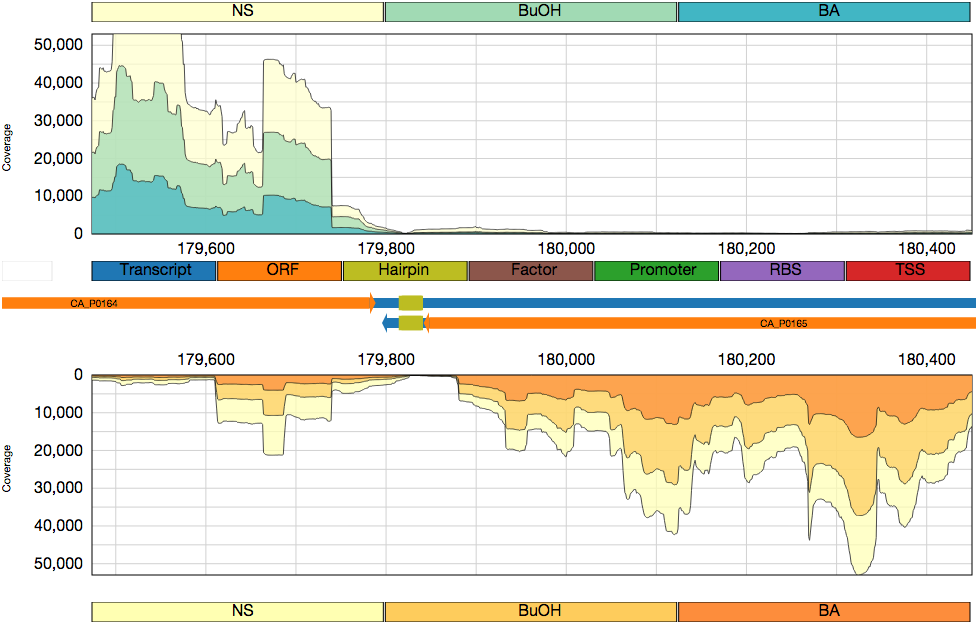
\includegraphics[width=\textwidth,height=2.5in]{images/Assembly/Examples/Sol/Sol-bifunctional-terminator.png}
\subcaption{Bifunctional Rho-independent terminator for Sol operon (upper track, left), Adc}\label{fig:2b}}
{\includegraphics[width=\textwidth,height=1.5in]{images/Assembly/Examples/Sol/Sol-Adc-curated.png}
\subcaption{Curated Adc locus}\label{fig:2c}}
\caption{Adc locus}
\subref{fig:2a}) Transcription initiation region for Adc. While the coverage clearly shows the appropriate increase, the transcription start site has been fused to residual coverage upstream of the true TSS. \subref{fig:2b}) A bifunctional terminator is responsible for transcriptional termination of both Adc and the Sol operon. \subref{fig:2c}) With minor curation, the region matches previous results faithfully.
\label{fig2}
\end{figure}


\paragraph{Sol Operon}
These studies additionally describe the Sol operon. In \cite{65}, Durre et al. examined the Sol operon using a probe specific for ctfB and reported a transcript size of 4.1kb. Unfortunately, no blots were included as figures in this work. In \cite{63} AdhE-based probes revealed a nearly identical transcript size of 4.1-4.2kb. Interestingly, the Sol operon has both proximal and distal transcription start sites at 175,726 and 175,564, respectively\cite{62,63}. Ribosome binding sites have been identified upstream of AdhE, CtfA, and CtfB\cite{63}. The expression level of the Sol operon is substantial, also upwards of 10,000x coverage cumulatively. The distal transcription start site is matched perfectly (\ref{fig:3a}), demonstrating the precision of the assembly technique in the absence of background or residual signal. An increase in coverage is observed immediately following the proximal promoter (\ref{fig:3a}) in close agreement with the previous determinations\cite{62,63}. However, the transcription stop site was not precisely determined by the assembly, owing in part to basal antisense signal from the Adc gene (\ref{fig:2b}). After adjustment, the transcript sizes are 4,115 and 4,277, respectively, in close agreement with the reported transcript sizes\cite{63,65}.

\begin{figure}
\small
{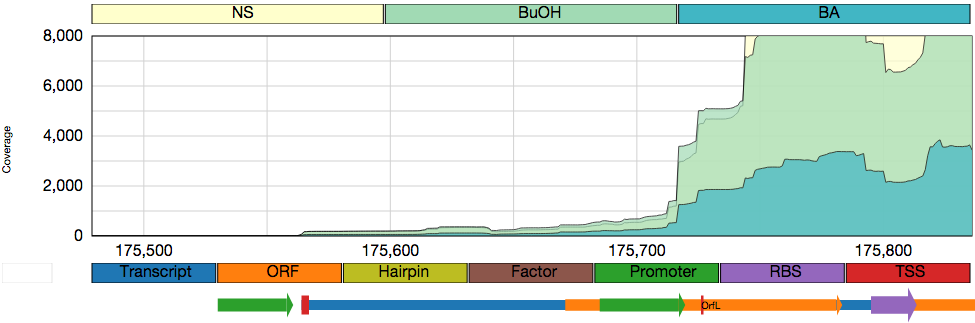
\includegraphics[width=\textwidth,height=1.5in]{images/Assembly/Examples/Sol/Sol-TSS.png}
\subcaption{Sol operon transcription initiation region. The distal (left) and proximal (right) transcription start sites (red) are shown for AdhE (far right, orange).}\label{fig:3a}}
{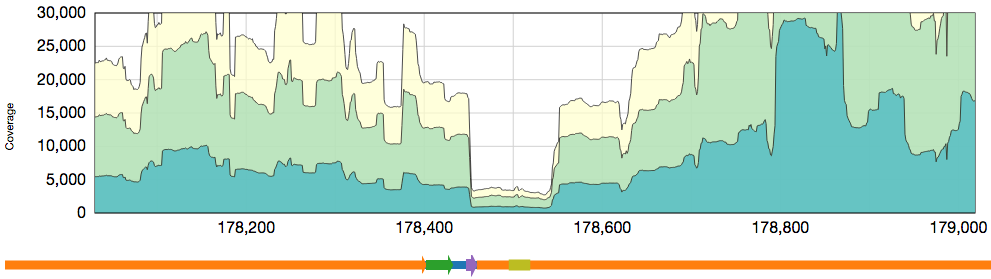
\includegraphics[width=\textwidth,height=1.5in]{images/Assembly/Examples/Sol/Sol-AdhE-terminator.png}
\subcaption{Putative AdhE (left) terminator, CtfA (right) promoter}\label{fig:3b}}
\caption{Sol Operon}
\subref{fig:3a}) Sol operon (OrfL, center; AdhE right) transcription start sites. The coverage and assembly data have strong agreement with previously described proximal and distal promoters and transcription start sites. \subref{fig:3b}) Low coverage in the Sol operon. A terminator may be partially responsible for a sustained low coverage level in the Sol operon. Additionally, a promoter motif was located upstream of the CtfA RBS and the pattern of expression is consistent with these observations.
\end{figure}

\paragraph{Multiple Transcripts from Sol Operon}
While the results from this region agree as a whole, there is an interesting pattern in coverage in the Sol operon near the C-terminus of AdhE(\ref{fig:3b}. This 100bp region is expressed at a statistically lower level (K.S.-test, p < 0.05) than the rest of the Sol operon. Upon further examination of this region, we find a Rho-independent terminator with a \(\Delta\)G of -9.6 kcal/mol, which is not as strong as the -11.5 kcal/mol bifunctional terminator at the end of the Sol operon. The region is also near a Sigma-A promoter motif of TTCATA(13)TATAAT located upstream of the previously mentioned RBS. As mentioned above, no Northern blots figures were included in the only study, to the best of my knowledge, that uses ctfA or ctfB specific probes\cite{65}. Most studies of the Sol operon in \textit{C. acetobutylicum} use AdhE-specific probes or larger restriction digestion probes \cite{63,68,70}. One of these displays a Northern with a weak but distinct band for a ~2.6kb transcript under solventogenic conditions \cite{68}. If AdhE were transcribed both in the classical Sol operon and as a separate transcript, the length would be 2,716bp from the proximal transcription start site. This pattern of coverage is consistent across all replicates. This length of the pattern suggests this observation does not merely represent difficulty sequencing secondary structure in the Sol operon transcript. In addition to the full Sol operon transcript, additional transcripts from the AdhE and ctfA/B genes may be produced.


\paragraph{SolR Transcript}
The last transcript produced from the Sol locus considered here is that of the SolR gene. This gene produces two transcripts, one 1kb and the other 1.3kb\cite{63}. A later study revealed the role of SolR as a repressor for the Sol operon\cite{67}. This study also produced a single transcription start site at 174,154 on the pSol1 plasmid. As a result of examining this dataset, we see a perfect recapitulation of the transcription start site (\ref{fig:4a}). The transcript from the raw assembly is approximately 1.2kb, showing only residual coverage (cumulatively \textless 5x) after the first terminator. After curation (\ref{fig:4b}), the transcript size is 1,036bp. There was insufficient coverage in the conditions studied to strongly support the larger transcript and no alternative transcription start sites were apparent.


% Transcription start sites SolR
\begin{figure}
{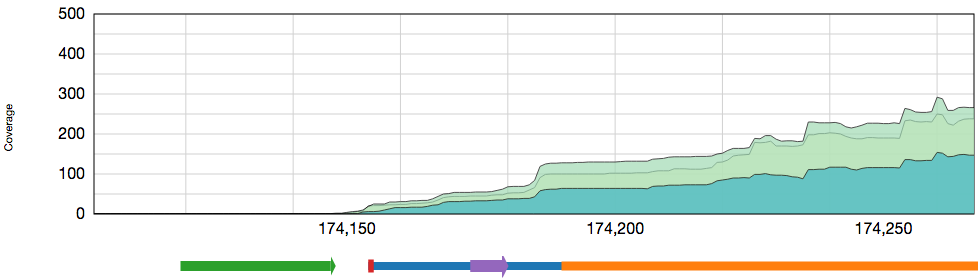
\includegraphics[width=\textwidth,height=1.5in]{images/Assembly/Examples/Sol/Sol-SolR-TSS.png}
\subcaption{SolR transcription initiation region}\label{fig:4a}}
{\includegraphics[width=\textwidth,height=1.5in]{images/Assembly/Examples/Sol/Sol-SolR-curated.png}
\subcaption{Curated SolR Transcript}\label{fig:4b}}
%\label{fig:1.5}
\caption{SolR Locus}
\subref{fig:4a}) The assembled transcription start site for SolR agrees with previous findings. \subref{fig:4b}) The curated SolR transcript agrees with previously published findings\cite{63,67}.
\end{figure}

\subsubsection{Bdh Locus}
The Bdh locus encodes two homologous butanol dehydrogenase(BDH) enzymes in a 3kb region on the main chromosome. Early studies of butanol dehydrogenases in \textit{Clostridia} located a number of NADH-dependent and NADPH-dependent BDHs and ADHs responsible for butanoate metabolism\cite{69,70,71,72}, specifically the reduction of butyryl and acetyl groups into the solvents butanol and ethanol. One such locus in \textit{C. acetobutylicum} produces two isozymes with different physiological roles. These isozymes like have distinct regulation and physiological roles from the other alcohol dehydrogenases found in this organism. The Bdh locus proteins were described by several authors, reporting different activities and specificities for each enzyme\cite{69,70}. After characterizing the enzymes in this locus, the region was cloned and two homologous isozymes were found. The two transcripts originating from these isozymes will demonstrate the precision and accuracy of this technique when compared to primer-extension analyses but also the need for assembly curation that reflects the motifs and coverage pattern of the region. We begin by discussing the first of these, BdhA.
\paragraph{BdhA}
BdhA is an NADH-dependent butanol dehydrogenase that acts on both butyryl and acetyl groups. Studies suggest that this enzyme has fairly comparable activities with both substrates, with slightly higher activities for butyryl groups\cite{70}. This enzyme was observed to have higher activities at low pH, indicative of its physiological role in the conversion of butyric acid to butanol. The entire locus was sequenced, producing ORFs that exactly matched the BdhA and BdhB isozymes\cite{72}. Northern analysis determined that these genes are transcribed separately and not as an operon. BdhA was found to have a 1.3kb transcript and the transcription start site was mapped through primer-extension to base 3,465,240 on the main chromosome of \textit{C. acetobutylicum}\cite{72}. Here we find the transcription start site of BdhA one base upstream at 3,465,241. The results of transcription start site identification agree well with the upstream Sigma-factor A promoter and the aforementioned start site. The uncurated assembly produces a transcription stop site at base 3,464,329, before the stop codon(\ref{fig:5b}). The pattern of coverage, however clearly reflects the Rho-independent terminator nearby. The final transcript reflects the assembly, coverage pattern, and motifs in this locus, agreeing with the transcription start site and a transcript length of 1,282bp. In this example, the fairly obvious coverage pattern was not reproduced by the assembly, demonstrating the need for some simple curation, integrating knowledge of previous experimental data and global predictions of promoter and terminator motifs with the coverage pattern and assembly.
%        B d h A
\begin{figure}
{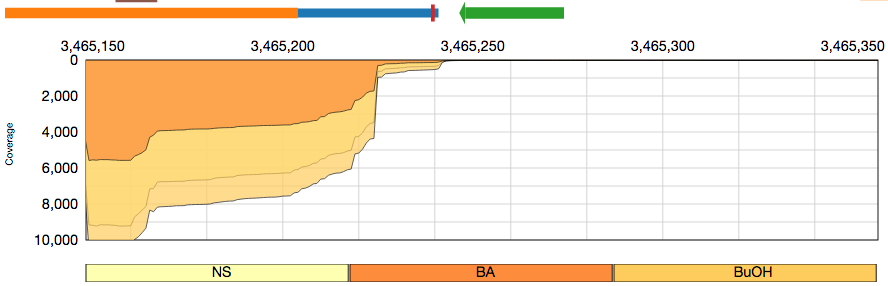
\includegraphics[width=\textwidth,height=1.5in]{images/Assembly/Examples/Bdh/BdhA-TSS.png}
\subcaption{BdhA Transcription Initiation Region}\label{fig:5a}}
{\includegraphics[width=\textwidth,height=1.5in]{images/Assembly/Examples/Bdh/BdhA-stop_site.png}
\subcaption{BdhA Transcription Termination Region}\label{fig:5b}}
{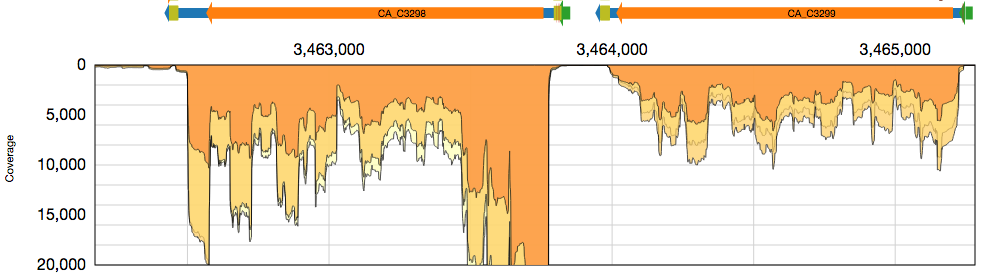
\includegraphics[width=\textwidth,height=1.5in]{images/Assembly/Examples/Bdh/Bdh-curated.png}
\subcaption{Curated BdhA Transcript}\label{fig:5c}}
\caption{Bdh Locus}
\subref{fig:5a}) The BdhA transcript displays a sharp increase in coverage near the transcriptional start site. This data agrees to a good extent with primer extension studies for this gene. \subref{fig:5b}) The raw assembly has failed to recapitulate the transcription termination region, likely due to low complexity coverage of the 3' region of this transcript. \subref{fig:5c}) The curated transcript reflects experimental characterization of this transcript\cite{72}.
\end{figure}

\paragraph{BdhB}
The next gene is BdhB, another NADH-dependent butanol dehydrogenase, with a slightly longer transcript size of 1.35kb. It was reported that this enzyme has 46-fold higher activity with butyryl groups than acetyl groups\cite{70,72}. BdhB was sequenced an analyzed along with BdhA, where it was discovered that BdhB had at least two transcription start sites, independent from BdhA. The most dominant transcription start site was very close to a secondary band at approximately 3,463,816 and 3,463,811, respectively\cite{72}. I will refer to these two distal bands collectively as the primary transcription start site for BdhB. A third band was located slightly farther upstream at 3,463,803\cite{72}. The coverage pattern for this region shows at least 3 sites of substantial increases in coverage at 3,463,802, 3,463,813, and 3,463,843 (\ref{fig:6a}). The first and proximal site has a promoter motif upstream, corresponding to the 1$^{st}$ -10 and -35 boxes in \ref{table:1} and the tertiary transcription start site\cite{72}. The second site has a significant increase in coverage between residue 3,463,817 and 3,463,810, which match well with the primary transcription start site described above\cite{72}. The primary transcription start site is explained by the 2$^{nd}$  -35 box and the 2$^{nd}$ or 3$^{rd}$ -10 box motifs\cite{72}. The final (distal) increase in coverage agrees with the 4$^{th}$ promoter motif(\ref{table:1}). It is clear that the strongest start site is the primary transcription start site previously described\cite{72}, although the multiple bands observed in their analysis could indeed be explained by matches to consensus Sigma-factor A motifs. Additionally, an observable but insignificant increase correlated with a final promoter motif. It is clear that the raw data match previous results to a good extent but curation was required to correct the transcription start site(\ref{fig:6a}) and stop site (\ref{fig:6b}). The final transcript is shown in \ref{fig:6c} with a final length of 1,367bp or 1,381bp, in close agreement with the published length of 1.35kb.

\begin{table}
\caption{BdhB Sigma-factor A boxes}\label{table:1}
\begin{minipage}[b]{2.5in}
\begin{center}
\begin{tabular}{|c|c|c|c|c|}\hline
\multicolumn{5}{c}{-35 box}\\\hline
Motif & Start & End & Sequence & p-value\\\hline
1 & 3463831 & 3463836 & TAGGTT & 3.5\e{-2}\\
2 & 3463847 & 3463852 & TTGTAA & 9.4\e{-3}\\
3 & 3463870 & 3463875 & TGGATA & 2.6\e{-2}\\\hline
\end{tabular}
\end{center}
\end{minipage}
\begin{minipage}[b]{2.5in}
\begin{center}
\begin{tabular}{|c|c|c|c|c|}\hline
\multicolumn{5}{c}{-10 Box}\\\hline
Motif & Start & End & Sequence & p-value\\\hline
1 & 3463816 & 3463821 & TATAAT & 4.3\e{-4}\\
2 & 3463820 & 3463825 & TATATA & 1.6\e{-3}\\
3 & 3463830 & 3463835 & TAAAAT & 4.2\e{-3}\\
4 & 3463852 & 3463857 & TATTAT & 4.2\e{-3}\\\hline

\end{tabular}
\end{center}
\end{minipage}
\end{table}
\begin{figure}
\small
{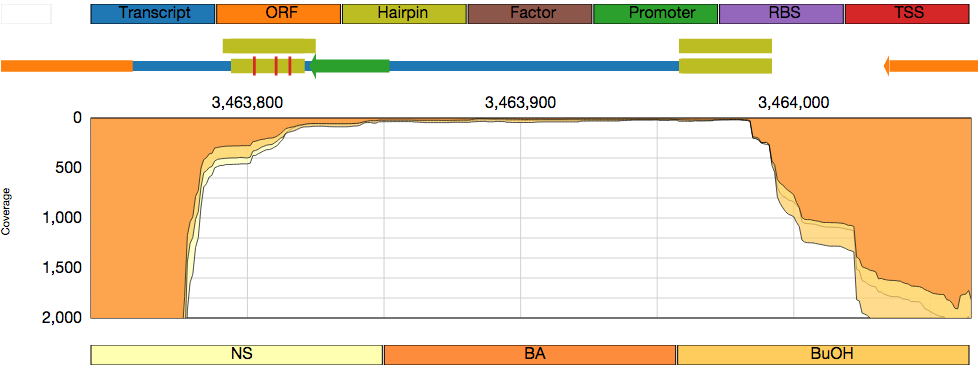
\includegraphics[width=\textwidth,height=1.5in]{images/Assembly/Examples/Bdh/BdhB-TSS.png}
\subcaption{BdhB Transcription Initiation Region}\label{fig:6a}}
{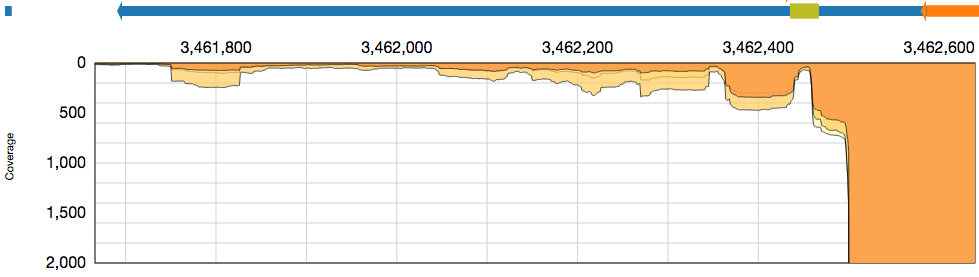
\includegraphics[width=\textwidth,height=1.5in]{images/Assembly/Examples/Bdh/BdhB-termination.png}
\subcaption{BdhB Transcription Termination Region}\label{fig:6b}}
{\includegraphics[width=\textwidth,height=1.5in]{images/Assembly/Examples/Bdh/BdhB-curated.png}
\subcaption{Curated BdhB Transcript}\label{fig:6c}}
\caption{Bdh Locus and Transcription Start Sites}
\subref{fig:6a}) The BdhB transcript has several promoter motifs and matching increases of coverage. These increases agree with previous experimental results\cite{72}, 2 of which were dismissed after not identifying the appropriate promoters. Unfortunately, the transcription start site was incorrect in the raw assembly. \subref{fig:6b}) A Rho-independent terminator is found at the end of the BdhB transcript although residual coverage triggered misassembly. \subref{fig:6c}) The final transcript matches previous results after integrating promoter and terminator motif information with the coverage pattern and assembly.
\end{figure}

In this example, the BdhA and BdhB transcripts were very close to capturing the true boundaries of these genes. In the case of BdhA the TSS was precise, but the assembled transcript did not match the coverage pattern or the ORF and terminator annotations. In the case of BdhB however, the start and stop sites did not agree with patterns in coverage and were simple to correct. The next example is another positive example, this time of a stress-response operon containing the heat-shock proteins GroES and GroEL.

\subsubsection{GroES/EL Locus}
\paragraph{GroES/EL Operon}
The GroES and GroEL proteins are evolutionarily conserved heat-shock responsive chaperonins. These proteins are found throughout the tree of life, including \textit{C. acetobutylicum}, where they are an integral to the solvent stress response\cite{73,74,75}. Additionally, evidence suggest that they are part of the class I heat-shock response in \textit{C. acetobutylicum}\cite{42}. Expression levels were very substantial for this region and a dramatic increase with solvent stress or heat shock was observed\cite{73,74}. In a molecular study, GroES and GroEL were found to be produced from a bicistronic operon with a transcript size of 2,150bp\cite{75}. In addition, a Sigma-factor A promoter was identified for an experimentally determined transcription start site. Two bands were observed during the primer-extension assay\cite{75}. The proximal band was dismissed as an artifact although the bands persisted under all conditions examined\cite{75}. This region is known to contain at least one CIRCE element upstream\cite{76} and one overlaps both of these start sites (\ref{fig:7a})\cite{74}. The transcription start site determined in this work is located at 2,829,142, a mere two bases away from the previously reported start site\cite{75} (\ref{fig:7a}). The second transcription start site is located at a sharp increase in expression. The distance of this start site from the promoter suggests post-transcriptional processing. The transcription stop site is located near a Rho-independent terminator (\ref{fig:6b}). The transcript size determined by the raw assembly is 2,131bp in agreement with the 2.2kb band and the 2,150bp calculated distance between the transcription start-site and the Rho-independent terminator\cite{75}. In this example, the uncurated assembly produced a flawless recapitulation of the coordinates and size of the GroES/EL operon (\ref{fig:6b}). Having established the coordinates for this transcript in agreement with previous findings, the regulation of this operon should be discussed.

\paragraph{GroES/EL Regulation}
The CIRCE element of the GroES/EL operon is regulated by the heat-shock repressor HrcA, the key regulatory protein for the class I stress response. HrcA is a temperature sensitive repressor that regulates class I genes through a canonical mechanism involving GroEL. GroEL is known to modulate HrcA activity through a titration mechanism involving misfolded proteins\cite{42,76,77}. Recently, an additional mechanism was discovered in \textit{H. pylori} where HrcA binding to CIRCE-elements is decreased at higher temperatures in comparison to other heat-shock regulators\cite{77}. Upon heat-shock or the generation of misfolded proteins, the GroES/EL operon is derepressed and the transcription activity increases acutely for 2-3 minutes, followed by a return to standard levels after 10 minutes\cite{76}. Cumulatively, we instead observe a general downregulation of the GroES/EL operon(\ref{fig:6b}). This is symptomatic of another portion of the stationary phase phenomena in \textit{C. acetobutylicum}, the 6S small RNA. The 6S small RNA titrates the Sigma-factor A, resulting in a subsequent downregulation of genes in the Sigma factor A regulon, including both the 6S and GroES/EL. We will revisit this locus in a subsequent differential expression analysis. The results presented here show excellent precision and accuracy in the determination of transcript coordinates.



\begin{figure}
\small
{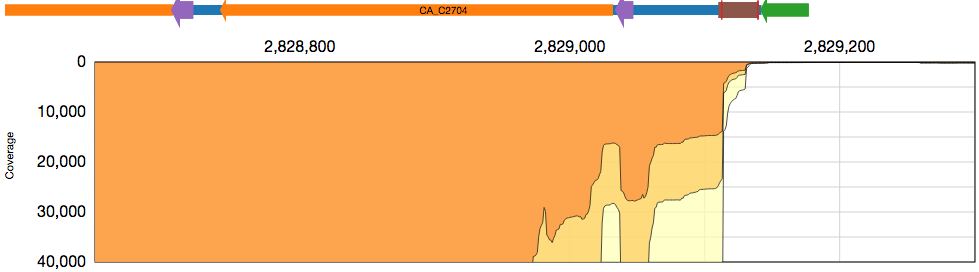
\includegraphics[width=\textwidth,height=1.5in]{images/Assembly/Examples/GroESL/GroESL-TSS.png}
\subcaption{GroES/EL Transcription Initiation Region}\label{fig:7a}}
{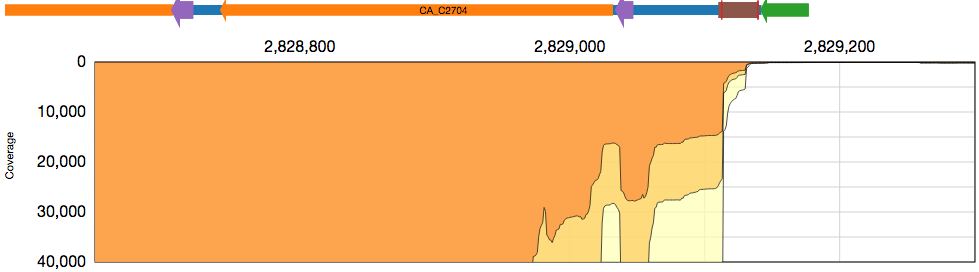
\includegraphics[width=\textwidth,height=1.5in]{images/Assembly/Examples/GroESL/GroESL-TSS.png}
\subcaption{GroES/EL Transcription Termination Region}\label{fig:7b}}
\caption{GroES/EL Locus}
\subref{fig:5a}) GroES and GroEL form an operon that is responsive to heat-shock through a HrcA-mediated derepression mechanism. The transcription start sites are in agreement with previous findings with the addition of an interesting peak inbetween these two. \subref{fig:5b}) The transcription termination region supports previous reports of a 2.2kb transcript terminating at a Rho-independent terminator following the GroEL ORF.
\end{figure}

%   H r c A,  G r p E,  D n a K,  &  D n a J
The final example that we consider with primer extension analysis is the HrcA operon. This rather complex locus encodes the class I repressor HrcA and DnaK and DnaJ, another set of evolutionarily conserved heat-shock proteins. DnaK was discovered to be solvent-stress responsive in \textit{C. acetobutylicum}\cite{73,74}. Solvent stress and heat shock share the critical issue of protein denaturation and require molecular chaperones such as GroES/EL and DnaK/J to increase proper protein folding in these conditions. The DnaK protein was first purified as a stress responsive 74kDa protein\cite{74}. Using a restriction fragment, the DnaK locus was cloned and sequenced, revealing a grouping of four ORFs\cite{79}. A similarly structured repeat was found upstream of HrcA, now known to be the HrcA-binding CIRCE element\cite{79}. 



\begin{table}
\caption{HrcA Operon Sigma-factor A boxes}\label{table:2}
\begin{minipage}[b]{2.5in}
\begin{center}
\begin{tabular}{|c|c|c|c|c|}\hline
\multicolumn{5}{c}{-35 box}\\\hline
Motif & Start & End & Sequence & p-value\\\hline
1 & 1423774 & 1423779 & ATGAAA & 5.3\e{-2}\\
2 & 1423790 & 1423795 & TTGACA & 2.9\e{-4}\\\hline
\end{tabular}
\end{center}
\end{minipage}
\begin{minipage}[b]{2.5in}
\begin{center}
\begin{tabular}{|c|c|c|c|c|}\hline
\multicolumn{5}{c}{-10 Box}\\\hline
Motif & Start & End & Sequence & p-value\\\hline
1 & 1423800 & 1423805 & TAATGT & 1.8\e{-2}\\
2 & 1423826 & 1423831 & TAGTCA & 1.5\e{-2}\\\hline
\end{tabular}
\end{center}
\end{minipage}
\end{table}

The HrcA locus consists of a polycistronic operon with multiple transcription start sites. The operon consists of the heat-shock program regulator HrcA, the nucleotide exchange factor GrpE, and the molecular chaperones DnaK and DnaJ. In an early study of this region, 4 transcripts were identified for this operon. The first was a 5kb transcript containing all 4 proteins. The second a 3.8kb transcript contains HrcA, GrpE, and DnaK while the third (2.6kb) contains only GrpE and DnaK. The final transcript contains DnaJ and is 1.4kb. One previously documented Rho-independent terminator has been described downstream of DnaK in \textit{C. acetobutylicum}.

In this dataset, the coverage pattern matches very well with the previously published transcript size of 5kb. Interestingly, the HrcA transcription start site determined by the uncurated assembly is comparable to previous studies. Moreover, the assembly predicts a transcription start site with reasonable accuracy, considering the level of residual signal from the upstream gene. The data could certainly reflect the transcriptional terminator downstream of DnaK, but no Rho-independent terminator was found downstream of DnaJ using three different algorithms. The termination of this transcript may be due to a non-intrinsic termination mechanism. This region has also been fused to signal from the downstream gene.

\begin{figure}
\small
{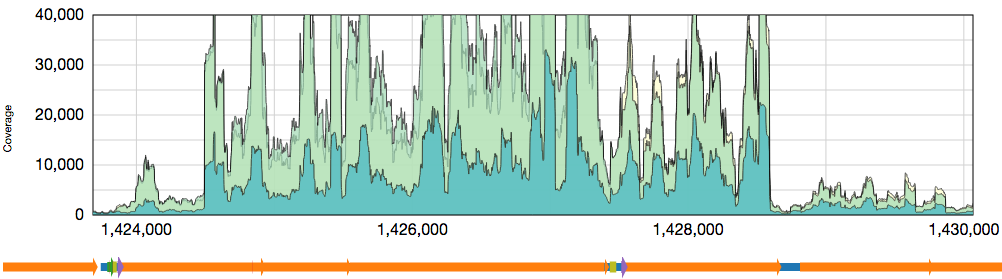
\includegraphics[width=\textwidth,height=1.5in]{images/Assembly/Examples/HrcA/HrcA-locus.png}
\subcaption{Operon consisting of HrcA, GrpE, DnaK, and DnaJ}\label{fig:7a}}
{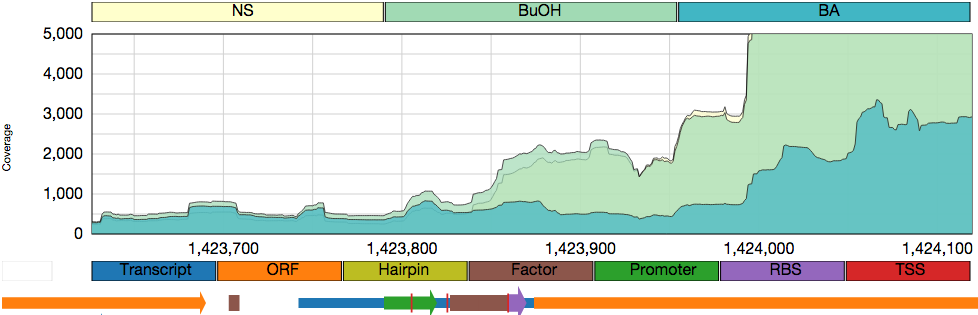
\includegraphics[width=\textwidth,height=1.5in]{images/Assembly/Examples/HrcA/HrcA-TSS.png}
\subcaption{HrcA transcription initiation region.}\label{fig:7b}}
{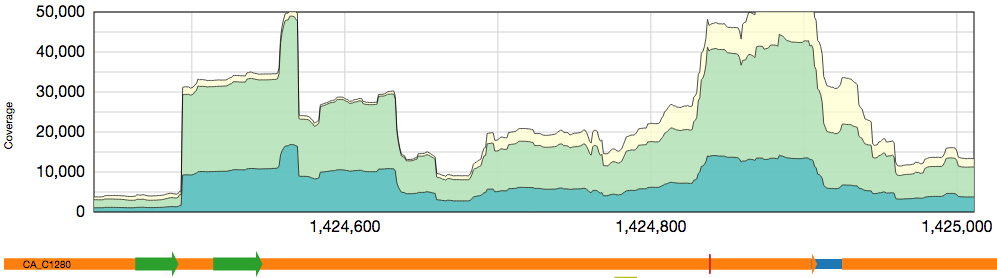
\includegraphics[width=\textwidth,height=1.5in]{images/Assembly/Examples/HrcA/GrpE-TSS.png}
\subcaption{GrpE transcription initiation region.}\label{fig:7c}}
{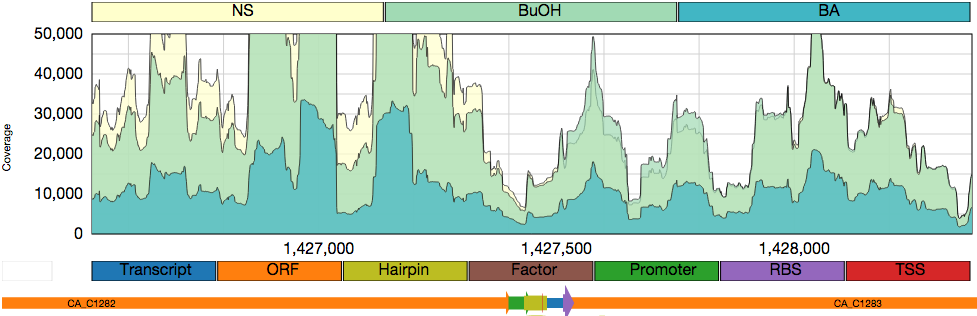
\includegraphics[width=\textwidth,height=1.5in]{images/Assembly/Examples/HrcA/DnaKJ-IGR.png}
\subcaption{DnaK-DnaJ IGR and DnaJ transcription initiation region}\label{fig:7d}}
\caption{HrcA locus}
\subref{fig:7a}) The highly expressed HrcA locus encodes several transcripts of different size. \subref{fig:7b}) The assembled transcription start site for the HrcA gene provides a reasonable estimate, considering the level of background signal for this region. \subref{fig:7c}) The transcription start site is not distinguishable in the coverage data. \subref{fig:7d}) The intergenic region between DnaK and DnaJ contains the only hairpin for this operon, which matches a decrease in coverage. The reported transcription start site is not identifiable from the coverage in this region.
\end{figure}

%          S p o 0 A

Spo0A is the master regulator of sporulation and stationary phase phenomena. This protein is thought to ultimately transduce growth-limiting and stressful signals into sporulation behavior in a number of anaerobic firmicutes. In previous studies, Spo0A was shown to be translated from a 0.9kb transcript in \textit{C. acetobutylicum}. Here we observe a slightly longer transcript of ~1.1kb according to the pattern of coverage. However, no Rho-independent terminators were found immediately downstream (\textless  200bp) of Spo0A, suggesting either a non-intrinsic termination mechanism or differing transcript sizes from those previously reported. Unfortunately, the boundaries represented by this coverage pattern were not detected due to the background signal in the area. Consequently, this region needs some remediation and is the first example of a completely fused transcript, not merely an extension.

In a nearby location, the genes CAC2073-2078 are found in a tight grouping near a large peak of expression. This peak correpsonds to an uncharacterized protein CAC2079 that is present in UniProt but absent from NCBI and KEGG databases. Its coverage appears to be largely above 20k per base, independent of the surrounding regions (although the transcript is indeed fused). Bioinformatic analysis suggests that it shares sequence similarity to proteins in the \textit{Clostridia}, \textit{Bacilli}, \textit{Baceteroidetes}, and \textit{Halobacteria}. While there was no common catalytic or active domain unifying this group of homologs, the region of homology tends to precede a transmembrane motif. Further analysis via PSI-blast result suggests sequence similarity to mATE (Multidrug And Toxic-compound Extrusion) efflux family proteins. mATE family proteins use electrochemical gradients to export antibiotics and other toxic compounds. The data suggest that the expression of this protein is important to \textit{C. acetobutylicum} and it will be interesting to examine the expression profile statistically. This instance demonstrates the synergy of older annotations with the newer coverage data and once again the need for semi-automated curation. Next we explore another stress-responsive region with a regulatory protein, the HrcA locus.

\begin{figure}
\small
{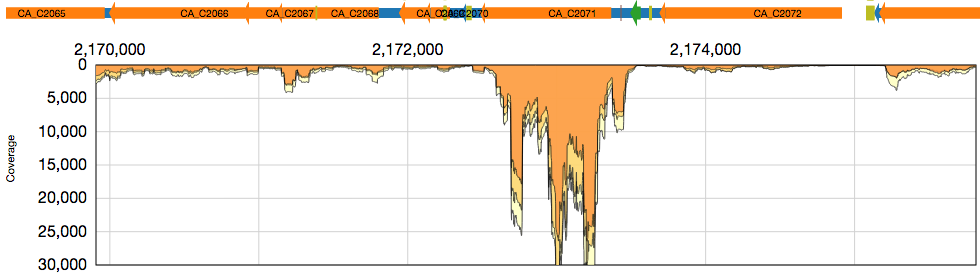
\includegraphics[width=\textwidth,height=1.5in]{images/Assembly/Examples/Spo0A/Spo0A-locus.png}
\subcaption{Spo0A transcript (center) fused to signal from neighboring regions}\label{fig:6a}}
{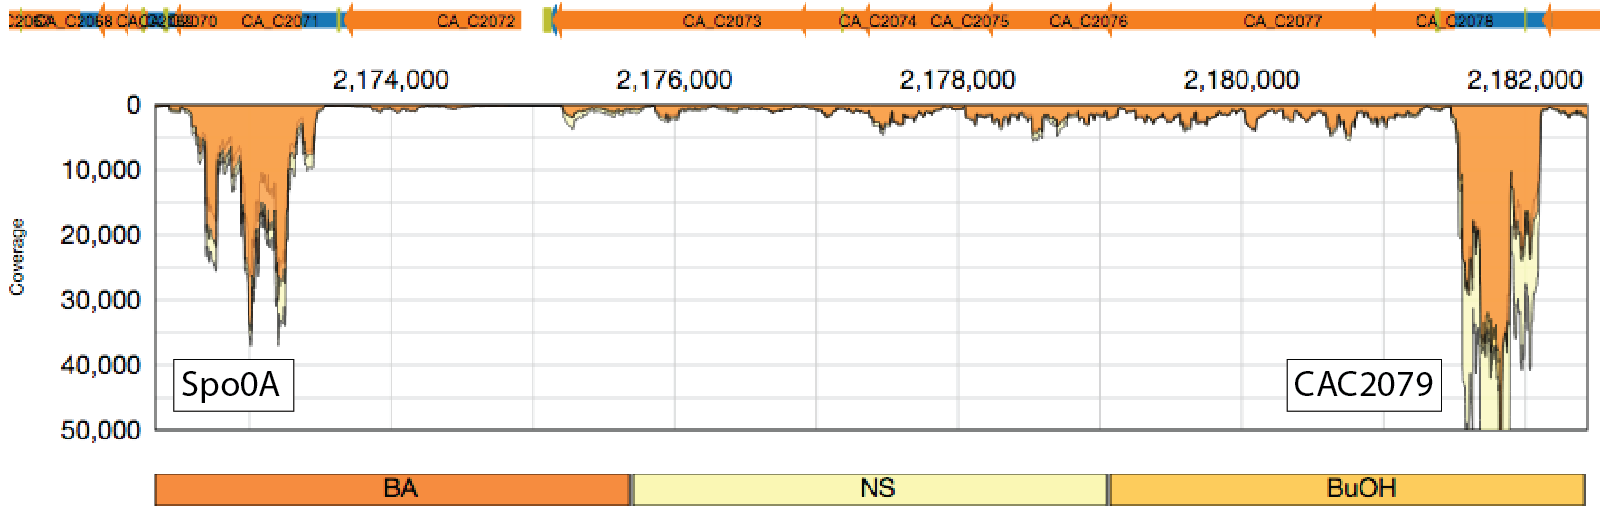
\includegraphics[width=\textwidth]{images/Assembly/Examples/Spo0A/CAC2079.png}
\subcaption{Upstream region of Spo0A, including CAC2079, a putative protein missing from many databases.}\label{fig:6b}}

\caption{Spo0A locus}
\subref{fig:6a}) The Spo0A transcript is found in a region of sufficient k-mer complexity and background coverage for the assembled transcript to be fused to signal from neighboring operons. This region clearly requires attention from curation strategies. \subref{fig:6b}) The region upstream of Spo0A consists of a late stage sporulation protein and a group of proteins in tight formation. Interestingly, there is a missing annotation in NCBI and KEGG for protein CAC2079 near a large peak of expression, in between the annotated proteins CAC2078 CAC2080.
\end{figure}


\subsection{Identify and Attempt to Resolve Remaining Issues}
There are two principal challenges relating to this uncurated transcriptome assembly. The first relates to the qualification of novel transcripts which I will defer to a later time. The second involves the curation of the 1057 transcripts which encode reference CDSes. After considering the examples above, we are left with a few types of misassembly to address.
\begin{enumerate}
\item Partial transcripts which overlap reference ORFs, but do not completely contain them. (e.g. BdhA)
\item Extended transcripts that possess larger UTRs than would be expected with respect to promoter and terminator motifs and coverage patterns. (e.g. Adc, CtfA/B)
\item Fused transcripts where the transcript from one gene is completely fused with signal from neighboring loci, with respect to prior knowledge, promoter, and terminator motifs (e.g. Spo0A).
\end{enumerate}

The first issue requires the simple solution of adjusting the transcript boundaries to include reference ORFs where there is not complete inclusion. Practically this requires only some minimal scripting and the use of '\href{http://bedtools.readthedocs.org/en/latest/content/tools/merge.html}{merge}' from bedtools, a toolkit for genomic set operations. The second issue requires a slightly more complicated solution of integrating information of regulatory motifs, terminators, and coverage information to find the solution that produces the most agreement between these various sources. In practice, I will integrate the various sources in the genome browser for context with the coverage information from this experiment. No completely automated tools exist to accomplish this. However, on average each transcript requires only a minimal amount of decision and should in principle be easy to curate. The third type of gene is completely fused to signal from other genes or noise. In the case of Spo0A, the true signal was simple to distinguish from noise, even in the absence of a Rho-independent terminator. In other cases the solution may not be so simple but contextual information about ontology combined with the various signals of coverage and stress response, promoters, and terminators make the problem more tractable. 

In principle, each of the pieces of information that I will integrate will not reproduce the transcript boundary on its own. In the examples above there are instances where the coverage alone fails to describe the transcript boundary, while the linguistic complexity of the dataset, used by the assembly algorithm, reproduces the boundary to a good extent. In other instances the opposite is true: a dramatic change in coverage near terminators or other signals is not recognized by the assembly alone. For that matter, there appear to be instances of non-intrinsic termination to complicate matters further. Therefore, these information are synergistic with respect to defining transcript boundaries and the absence of one signal may be made up for by the presence of another.

\subsection{Novel Transcripts}

\subsection{Exploratory Tools}


